%!TEX root = ../thesis.tex

\section{実験の概要}

  本研究では,2DLiDARの反射強度を利用したルールベース制御器を用いた人追従行動を,カメラ画像で模倣学習することを課題としている.ルールベース制御器は,最大反射強度の方にロボットが追従する手法となっているため,実験で使用する再帰反射テープよりも高い反射強度を取得してしまうと人追従行動を継続できない恐れがある.そこで,2DLiDARの反射強度の実験と提案手法による人追従の実験の2つに分けて実施する.それぞれの実験の概要を以下に示す.

  \subsubsection*{<実験1:2DLiDARの反射強度の実験>}
  \begin{itemize}
    \item 壁の反射強度を計測する実験
    \item 再帰反射テープの反射強度を計測する実験
    \item 学習フェーズで使用する周辺環境の反射強度を計測する実験
    % \item ルールベース制御器を用いた人追従の実験
  \end{itemize}
  
\newpage

  \subsubsection*{<実験2:提案手法による人追従の実験>}
  ルールベース制御器により10個の学習モデルを作成し,それぞれの学習モデルに対してテストを行う.つまり,実験を10回繰り返し,提案手法の有効性を検証する.

  \vspace{1cm}

  実験環境は,\figref{Fig:RobotGuidance_cit3f}に示すように千葉工業大学津田沼キャンパス2号館3階の廊下を使用した.実験は天候による影響を少なくするため,夜間に実施した.また,服装による影響を少なくするため,追従対象者は\figref{Fig:Sequence of the experiment}に示すような青いビブスを着用し,学習フェーズと追従フェーズに分けて実験を行った.

  \begin{figure}[h]
    \centering
    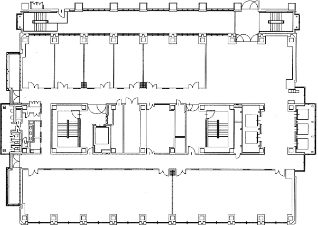
\includegraphics[keepaspectratio, scale=0.70] {images/RobotGuidance_cit3f.png}
    \captionsetup{justification=raggedright} % キャプションを左寄せに
    \caption{The environment of the experiment}
    \label{Fig:RobotGuidance_cit3f}
  \end{figure}

  \begin{figure}[h]
    \centering
    \begin{minipage}[c]{65mm} 
        \centering
        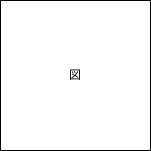
\includegraphics[height=40mm]{images/figure.png}
        \subcaption{Learning phase}
    \end{minipage}
    \begin{minipage}[c]{65mm} 
        \centering
        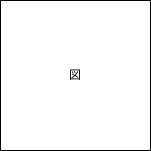
\includegraphics[height=40mm]{images/figure.png}
        \subcaption{Following phase}
    \end{minipage}
    \caption{Sequence of the experiment}
    \label{Fig:Sequence of the experiment}
  \end{figure}

\newpage
